%----------------------------------------
% IT IS RECOMMENDED TO USE AUTOLATEX FOR
% COMPILING THIS DOCUMENT.
% http://www.arakhne.org/autolatex
%----------------------------------------

\documentclass[english,nodocumentinfo,nopubpage]{utbmciadreport}

% The TeX code is entering with UTF8
% character encoding (Linux and MacOS standards)
\usepackage[utf8]{inputenc}
\usepackage{fancyhdr}
\usepackage{../common/sarl-colorized-listing}


\graphicspath{{./}}

\declaredocument{Introduction to SARL}{Tutorial Session \#4}{UTBM-INFO-AI51-TU4}

\addauthorvalidator*[St\'ephane Galland]{St{\'e}phane}{Galland}{Teacher}

\updateversion{1.0}{\makedate{20}{03}{2023}}{First release on Github}{\upmpublic}

\begin{document}

\section{Goal of this Tutorial Session}

The goal of this tutorial session is to introduce the implemention of a simple and general architecture for agent-based simulation. This architecture may be used for creating any simulator upon SARL technologies.

The goal of this session is to create a simulator that is running a collection of agents who are moving randomly on a 2D space.


\section{Work to be Done during the Tutorial Session}

\subsection{Step 1 - Environment Model}

The goal of this step is to implement the environment, which is part of the general architecture of an agent-base simulator, as illustrated on Figure \ref{fig:architecture}. The environment model is a class (in term of object oriented programming) that contains all the objects that are inside the simulated virtual world. Each agent is associated to a body, which is located in the environment. According to the lecture's slides, the agent environment has the mission to compute the collection of the objects in the fields of view of each agent (perception mechanism). The agent environment has also the mission to change the position of the agents' bodies on the environment.

\begin{figure}
	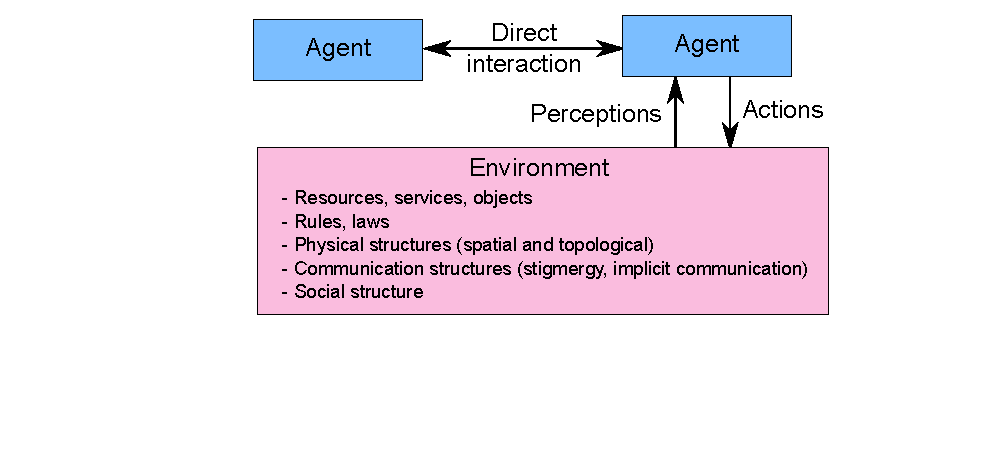
\includegraphics[width=\linewidth]{mabs_overview_layer1}
	\caption{General simulator architecture}
	\label{fig:architecture}
\end{figure}

\begin{enumerate}[a)]
\item Define a class named \code{Body}\ representing an agent body. This class must contains at least:
	\begin{itemize}
	\item the identifier (of type \code{UUID}) of the body, which is the same as the associated agent's identifier.
	\item the 2D position represented by two floating point numbers, \code{x}\ and \code{y}.
	\end{itemize}
\item Define a class \code{EnvironmentModel}\ that is a container of agent bodies and represents the 2D world in which the agents are evolving. This class must contains at least:
	\begin{itemize}
	\item a collection of agent bodies. You have to select the best type of collection for storing the agent bodies.
	\end{itemize}
\end{enumerate}

\subsection{Step 2 - Agent Perception}

Agent perception is the mecanism, implemented into the agent environment, that compute the collection of all the objects that are inside the virtual field of view of each agent.
In other word, each agent is equiped with a field of view (usually a circle centered on the agent position, with a radius which is representing a perception distance). Then, all the objects that are located in the field of view are considered to be perceived by the agent which is located at the center of this field. The collection of the perceived objects is computed to be provided to the agent.

\begin{enumerate}[a)]
\item In the class \code{EnvironmentModel}, define the function below that is computed the perceptions for each agent body stored in the environment model:
	\begin{center}
		\code{def computePerceptions : Map<UUID, List<Body>>}
	\end{center}
\end{enumerate}

\subsection{Step 3 - Agent Action}

Each agent is supposed to act in the environment. In this tutorial session, the agents are supposed to move on a 2D space. In order to apply the motion decisions of the agents, it is necessary to implement a function in the environment that change the positions of the agents.

\begin{enumerate}[a)]
\item Define the class \code{Motion}\ that describes a desire of motion from an agent. This class must contains at least:
	\begin{itemize}
	\item the identifier of the agent which has computed the motion.
	\item the 2D motion represented by two floating point numbers, \code{x}\ and \code{y}. The length of the vector \code{(x, y)}\ represents the distance to move to.
	\end{itemize}
\item In the class \code{EnvironmentModel}, define the function below that is applying the motions from the agents:
	\begin{center}
		\code{def applyAgentMotions(motions : Collection<Motion>) : void}
	\end{center}
\end{enumerate}

\subsection{Step 4 - Agent Environment Agent}

In order to implement the connection between the environment and the agent (see Figure \ref{fig:architecture}) is an easy way, we recommend to enclosing the environment model inside a dedicated agent, named the ``Agent Environment Agent''. This choice will enable us to have benefits of the event-exchange tools that are provided by the SARL programming language to all the agents.

Basically, the simulation process is an infinite loop during which each simulation step is composed by:
\begin{enumerate}[1)]
\item the computation of the perceptions for each agent;
\item the computation of the motion decision by each agent;
\item the motion of each agent in the environment.
\end{enumerate}

The following tasks must be done for implementing a runnable agent environment agent:
\begin{enumerate}[a)]
\item Define the SARL event with name \code{Perception}, that contains at least:
	\begin{itemize}
	\item The collection of perceived objects for an agent body.
	\item The reference to the agent body that is perceiving the objects above.
	\end{itemize}
\item Define the SARL event with name \code{AgentMotion}, that contains at least:
	\begin{itemize}
	\item A motion of type \code{Motion}.
	\end{itemize}
\item Define an agent with the name \code{AgentEnvironmentAgent}.
\item Define a function named \code{simulationLoopStart}\ that is:
	\begin{itemize}
	\item Compute the perceptions for all the agent body (see Step 2);
	\item For each agent body:
		\begin{itemize}
		\item Create an instance of event \code{Perception},
		\item Emit the create event to the agent with the same identifier as the identifier of the agent body, which is stored in the \code{Perception}\ event.
		\end{itemize}
	\end{itemize}
\item Define an event handler that is reacting to an event of type \code{AgentMotion}\ and that is:
	\begin{itemize}
	\item Applying the motion provided in the event in the environment model.
	\end{itemize}
\end{enumerate}


\subsection{Step 5 - Agent Behavior}

The agents whic hare moving must defined. Basically, each agent is computing a motion when it is receiving an update of its perception. That's why, we have to define the function for sending to the agent environment the motion computed by the each, and computing the motion when receiving a perception event from the agent environment.

\begin{enumerate}[a)]
\item Define an agent with the name \code{MovingAgent}.
\item In this agent type, define the function below that is emitting an event of type \code{Motion}\ to the agent environment agent:
	\begin{center}
	\code{def move(x; double, y : double) : void}
	\end{center}
\item Define an event handler that is reacting to an event of type \code{Perception}\ and that is:
	\begin{itemize}
	\item Computing a 2D motion that may be computed randomly, or simply by implementing the ``social force model'' explains in the lecture's slides.
	\item Calling the function \code{move}\ with the 2D motion.
	\end{itemize}
\end{enumerate}


\subsection{Step 6 - Start the Simulator}


For starting the simulator, we must implement a pieace of code in the agent \code{AgentEnvironmentAgent} (usually when it is starting) for creating the environment model, create a predefined number of bodies, spawn the associated agents, and start the simulation loop.

In this step, you have to take care of the parallel execution of the different functions.


\end{document}
